\title{COM S 352 Homework 4}
\author{Alec Meyer}

\date{\today}

\documentclass[11pt]{article}
\usepackage{changepage}
\usepackage{graphicx}
\usepackage{amsmath}
\graphicspath{ {./images/} }
\newcommand\tab[1][1cm]{\hspace*{#1}}
\usepackage{amssymb}


\begin{document}
\maketitle

\section*{Question 1}
\textbf{I/O-bound}: will have voluntary context switches because
a process will need a resource that is currently being used
when it gives up CPU control.\\
\textbf{CPU-bound}: will have non-voluntary context switches because when
its time slice has expired or is preempted by another
process it will be removed from its current process.

\section*{Question 2}
\textbf{First-come, first-served}: This cannot result in starvation because
everything in the datastructure will be touched eventually.\\
\textbf{Shrotest job first}: This can result in starvation because the
longer processes will have to wait longer which could cause them 
to starve.\\
\textbf{Round robin}: This cannot result from starvation because each
process has equal prority and will have equal times.\\
\textbf{Priority}: This can result in starvation because lower priority
processes will never be touched, causing them to starve.

\section*{Question 3}
\textbf{a.}\\
This formula will always take 100ms to predict the next CPU burst.\\
\textbf{b.}\\
$0.5t_n + 0.5T_{n+1}$\\
If the CPU burst is 30 milliseconds the resulting time will be 
20 milliseconds\\
\textbf{c.}\\
Most recent process behavior is given higher priority since the 
formula is $t_n$ milliseconds.

\section*{Question 4}
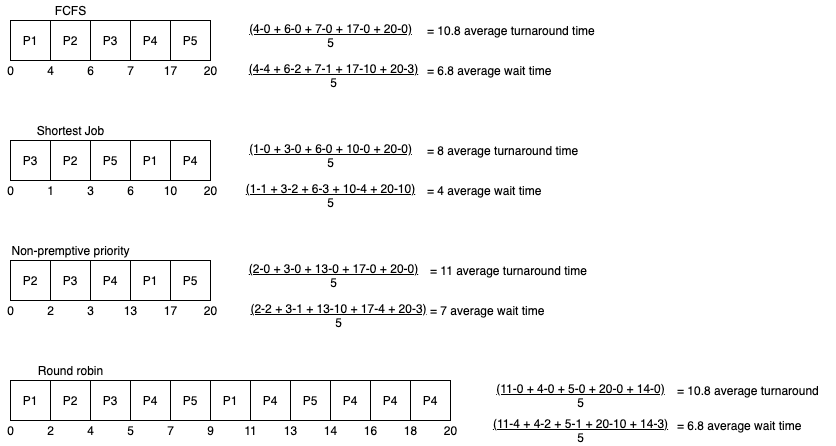
\includegraphics[scale=0.55]{COMS352HW4Q4.png}

\section*{Question 5}
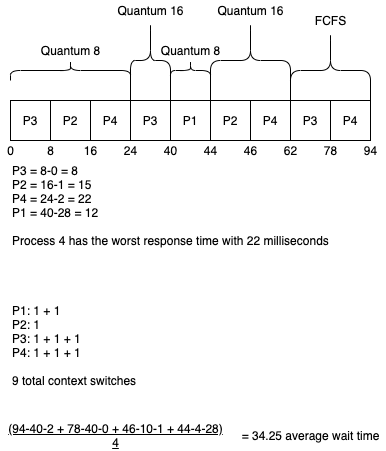
\includegraphics[scale=0.55]{COMS352HW4Q5.png}

\section*{Question 6}
\textbf{a.}\\
A has a higher priority vruntime will move slower, since they are 
CPU bound they will vruntime will be smaller for A.\\
\textbf{b.}\\
A will require less CPU time than B\\
\textbf{c.}\\
B will use the CPU less than A
\end{document}
